\documentclass[11pt]{article}
\usepackage[T1]{fontenc}
\usepackage{lmodern,microtype}
\usepackage[letterpaper,margin=1in]{geometry}
\usepackage{amsmath,amssymb,amsthm,mathtools,booktabs}
\usepackage{tikz}
\usepackage{xcolor}
\definecolor{inkblue}{HTML}{184E63}
\definecolor{copper}{HTML}{9B4829}
\usepackage[colorlinks=true,linkcolor=inkblue,citecolor=inkblue,urlcolor=inkblue]{hyperref}
\hypersetup{pdftitle={When Does a Field Have Ports?},
  pdfsubject={A graduate introduction to tensor wire prices and port graphs}}
\urlstyle{same}
\newtheorem{theorem}{Theorem}[section]
\newtheorem{proposition}[theorem]{Proposition}
\newtheorem{lemma}[theorem]{Lemma}
\newtheorem{corollary}[theorem]{Corollary}
\theoremstyle{definition}
\newtheorem{definition}[theorem]{Definition}
\newcommand{\F}{\mathbb F}
\newcommand{\R}{\mathbb R}
\newcommand{\E}{\mathbb E}
\newcommand{\one}{\mathbf 1}
\newcommand{\Var}{\mathcal V}
\newcommand{\En}{\mathcal E}
\newcommand{\res}{\longrightarrow}
\newcommand{\Gten}{\mathsf T}
\newcommand{\src}{\mathsf{Inc}}
\newcommand{\tgt}{\mathsf{Non}}
\newcommand{\Gr}{\operatorname{Gr}}
\newcommand{\rank}{\operatorname{rank}}
\newcommand{\fieldstatus}{27 November 2026}
\setlength{\emergencystretch}{1em}
\raggedbottom

\title{When Does a Field Have Ports?\\
An introduction to tensor wire prices}
\author{}

\AddToHook{cmd/maketitle/after}{%
  \par\noindent\begin{minipage}{\linewidth}
  \small\sffamily
  I asked ChatGPT these questions to understand what follows from the recent
  VP versus VNP breakthrough. I share its answers so that these explorations
  are available beyond a private conversation. These are AI-generated notes,
  not research papers. I do not claim authorship or priority for the ideas.
  Arguments may be wrong, and earlier work may be overlooked or misattributed.
  I welcome corrections by mail or via
  \href{https://github.com/radomite/algebraic-complexity/issues}{GitHub}.
  \end{minipage}\par\medskip
}
\AddToHook{shipout/foreground}{%
  \ifnum\ReadonlyShipoutCounter>1\relax
  \put(0pt,-24pt){\makebox[\paperwidth][c]{%
    \normalfont\sffamily\fontsize{8}{10}\selectfont\color[gray]{0.38}%
    AI-generated exploration notes. Arguments and attributions may be wrong.
    \href{https://github.com/radomite/algebraic-complexity/issues}{Corrections welcome on GitHub.}}}%
  \fi
}

\begin{document}
\maketitle

\section{Two edges across a cut}
\label{sec:cycle}

Seat \(2m\) terminals around a circle, with \(m\ge2\). Give the first \(m\) the value zero
and the next \(m\) the value one. Pick two terminals independently and
uniformly. Their values differ with probability \(1/2\). Now pick a random
edge of the circle. Its endpoints differ with probability only \(1/m\)
because exactly two edges cross the cut. We have arranged for a typical pair to
notice a separation that a typical edge almost always misses.

\begin{center}
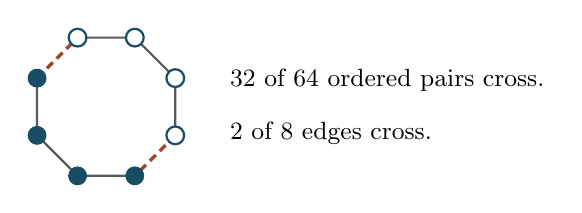
\begin{tikzpicture}[x=1cm,y=1cm]
  \foreach \i in {0,...,7} \coordinate (v\i) at ({112.5-45*\i}:0.95);
  \draw[thick,black!65] (v0)--(v1)--(v2)--(v3) (v4)--(v5)--(v6)--(v7);
  \draw[copper,densely dashed,very thick] (v3)--(v4) (v7)--(v0);
  \foreach \i in {0,...,3}
    \filldraw[fill=white,draw=inkblue,thick] (v\i) circle (3.2pt);
  \foreach \i in {4,...,7}
    \filldraw[fill=inkblue,draw=inkblue] (v\i) circle (3.2pt);
  \node[anchor=west,align=left,font=\small] at (1.45,.34)
    {\(32\) of \(64\) ordered pairs cross.};
  \node[anchor=west,align=left,font=\small] at (1.45,-.34)
    {\(2\) of \(8\) edges cross.};
\end{tikzpicture}
\end{center}

Why compare these experiments? Compressing a tensor network can collect many
wires at one vertex. Its attachment sites are called \emph{ports}. Replacing
the vertex by a graph on these sites spreads out its degree. The dense
comparison can inspect every pair of attachment sites. Its sparse
replacement can inspect only edges. We want the latter average to control
the former, with a factor independent of the number of sites.
This is the use of ports in the network compression argument of
\cite{euclid}.

There is a second reason to ask which fields have ports. Suppose we want
to count copies of a \(k\)-vertex expander in a weighted graph on \(n\)
vertices. Ruling out ports in a single characteristic would give, over
that characteristic, a family of maximum-degree-six expanders whose
induced counts require \(n^{\Omega(k/\sqrt{\log k})}\) arithmetic gates
in the fixed-pattern limit. How does a statement about the price of a
wire reach a counting problem? Section~\ref{sec:patterns} follows the
reduction and explains how far it gets toward an exponent \(ck\).

The interesting choice is what a separation should cost. In the example it
costs one to cross the cut and zero to stay on the same side. For a field
\(F\), there is a whole class of costs that arise from linear algebra over
\(F\). The graph must work for all of them simultaneously. If \(d_{ij}\)
denotes the cost of one bit shared between terminals \(i\) and \(j\), the
desired inequality is
\[
    \E_{\text{uniform pair }i,j}\,d_{ij}^{\,2}
    \ \le\ \gamma\,\E_{\text{uniform directed edge }i,j}\,d_{ij}^{\,2}.
\]
The circle forces \(\gamma\ge m/2\). To understand which graphs might
keep \(\gamma\) bounded, we first need to know which tables \(d_{ij}\)
linear algebra permits.

\section{How to price a wire}
\label{sec:prices}

Fix \(n\ge2\) labelled sites. A tensor over \(F\) is an array with an index
at each site, or, in basis-independent language, an element of
\(V_1\otimes\cdots\otimes V_n\) for finite-dimensional \(F\)-vector spaces
\(V_i\). An unused site has dimension one. Write \(S\res T\) if there are
linear maps \(A_i\) on the individual sites with
\((A_1\otimes\cdots\otimes A_n)S=T\). We say that \(S\) \emph{restricts}
to \(T\), or that \(S\) \emph{supplies} \(T\). Each site can mix all its own
indices. A wire is how two sites share an index.

Specifically, the \emph{binary wire} \(W_{ij}\) puts the matrix
\[
                 W(s,t)=\one_{\{s=t\}},\qquad s,t\in\{0,1\},
\]
at sites \(i,j\). The two labels index basis vectors over the chosen field
\(F\). As a tensor it is \(e_0\otimes e_0+e_1\otimes e_1\).
We can join the wires \(W_{ij}\) and \(W_{jk}\) by applying the linear
functional \(e_s\otimes e_t\mapsto\one_{\{s=t\}}\) at \(j\). The resulting
entry is \(\sum_t W(a,t)W(t,b)=W(a,b)\). Thus
\begin{equation}
                  W_{ij}\otimes W_{jk}\res W_{ik}.
                  \label{eq:splice}
\end{equation}
Here and throughout, tensor products group together all factors at the same
site. Each wire in such a product carries an independent bit.

A \emph{spectral point} \(\phi\) assigns a nonnegative real value to every
tensor on these sites over \(F\) according to the rules
\begin{align*}
 \phi(0)&=0,\qquad \phi(1)=1,\\
 \phi(S\otimes T)&=\phi(S)\phi(T),\qquad
 \phi(S\oplus T)=\phi(S)+\phi(T),\\
 S\res T&\quad\Longrightarrow\quad \phi(S)\ge\phi(T).
\end{align*}
Here \(1\) is the one-entry array \((1)\). A direct sum \(S\oplus T\) puts
the two arrays in disjoint coordinate blocks at every site and fills the
mixed blocks with zeros. For matrices this is the familiar block diagonal
sum. These rules define Strassen's asymptotic spectrum \cite{strassen-spectrum}.

Every nonzero tensor supplies \(1\) by selecting a nonzero entry and
rescaling. Fix a unit \(s>0\). Its \emph{price}
\(h(T)=s\log_2\phi(T)\) is therefore nonnegative, and products add
prices. The normalized unit is \(s=1\). Set \(d(i,j)=h(W_{ij})\) and
\(d(i,i)=0\). Equation~\eqref{eq:splice} gives
\(d(i,k)\le d(i,j)+d(j,k)\). We call \(d\) a \emph{wire distance}.
Distinct sites may have distance zero. A \emph{spectral placement} on
finitely many labelled terminals gives such a table of distances, using
one spectral point and one unit for all pairs. A placement that puts all
terminals at the same site gives the zero table. This
finite-table description suffices for the definition of ports
\cite{euclid}.

\paragraph{The circle's prices really exist.}
For a nontrivial cut \(S\mid S^c\), put all the indices from \(S\) on the
rows of a matrix and the others on its columns. The rank of this matrix
is a spectral point. Block diagonal ranks add, Kronecker product ranks
multiply, and applying local maps can only decrease rank. A crossing wire
has rank two. A wire with both ends on one side has rank one. Its price is
therefore exactly the zero-or-one cost in Section~\ref{sec:cycle} in
the normalized unit, over
every field, including in characteristic two.

\paragraph{A graph is also a tensor.}
Given a loopless multigraph \(H\), put a wire on each edge, including its
multiplicity, and write \(\Gten(H)=\bigotimes_{ij\in E(H)}W_{ij}\).
The price of the product and its rank across a cut are
\begin{equation}
 h(\Gten(H))=\sum_{ij\in E(H)}d(i,j),\qquad
 \rank_{S\mid S^c}\Gten(H)=2^{|\partial_H S|}.
 \label{eq:graph-price}
\end{equation}
Here \(\partial_H S\) denotes the edges crossing the cut. The first sum
uses distances to the \emph{first} power because it prices a product of
wires. The \emph{squares} in the port inequality measure the spread of a
placement.

\section{The definition and its Euclidean benchmark}
\label{sec:definition}

Let \(G\) be a \(d\)-regular undirected multigraph on \(n\) vertices, with
\(d\ge1\). Its transition matrix \(P\) gives each incident arc probability
\(1/d\), counting parallel arcs with multiplicity. A holding arc stays at
its vertex and counts once toward the degree. For a placement with
distances \(d_{ij}\), define
\begin{equation}
 \Var=\frac1{n^2}\sum_{i,j}d_{ij}^2,\qquad
 \En_G=\frac1n\sum_{i,j}P_{ij}d_{ij}^2.
 \label{eq:energy}
\end{equation}
The first experiment chooses two independent uniform vertices, allowing
the same vertex twice. The second starts at a uniform vertex and takes
one step. Both quantities have the same units, so rescaling a placement
preserves their ratio.

\begin{definition}[Ports {\cite{euclid}}]\label{def:ports}
A field \(F\) \emph{has ports} if there are constants \(D<\infty\) and
\(\gamma<\infty\) and regular undirected multigraphs of unbounded order,
each of degree at most \(D\), such that
\[
                       \Var\le\gamma\,\En_G
\]
for every graph \(G\) in the family and every spectral placement over \(F\)
of its vertices.
\end{definition}

The graphs and the two constants are chosen before the placements. A
disconnected graph fails on the cut separating one component from the
rest. For connected \(G\), let \(\Gamma_F(G)\) be the supremum of
\(\Var/\En_G\) on placements of positive diameter. The cycle computation
gives \(\Gamma_F(C_{2m})\ge m/2\). The complete graph \(K_n\) has
\(\Gamma_F(K_n)=(n-1)/n\), since its random edge is a uniform ordered
pair conditional on distinct endpoints. Its degree is \(n-1\).

The square still gives information about actual wires. Suppose a
permutation \(\pi\) specifies a destination for each terminal. For each
\(i\), compare \(i\) to \(\pi(i)\) through a uniform intermediate vertex
\(j\). The triangle inequality and Cauchy--Schwarz give
\[
 \frac1n\sum_i d_{i,\pi(i)}
   \ \le\ \frac{2}{n^2}\sum_{i,j}d_{ij}
   \ \le\ 2\sqrt{\Var}\ \le\ 2\sqrt{\gamma\En_G}.
\]
Thus one edge-energy estimate controls the per-terminal wire price for
every choice of destinations obtained by permuting the terminals.

\paragraph{Where ordinary expanders enter.}
Put real numbers \(f_i\) on the vertices, with their usual distance, and
subtract their mean. Directly expanding the squares in
\eqref{eq:energy} gives
\[
  \Var=\frac2n\|f\|_2^2,\qquad
  \En_G=\frac2n f^{\mathsf T}(I-P)f.
\]
The constant vectors have eigenvalue one for \(P\). Its largest eigenvalue
on the mean-zero subspace is denoted by \(\lambda_2(P)\). The best
constant for real placements is exactly \(1/(1-\lambda_2(P))\), by the
spectral theorem for symmetric matrices. Summing this calculation over
coordinates gives the same bound for vectors in any Euclidean dimension.
A bounded-degree family with \(1-\lambda_2(P)\) bounded below by a
positive constant is an ordinary \emph{expander family}.

Every finite Euclidean placement is spectral up to scale over every
coefficient field. This is a substantial theorem about tensors
\cite{euclid}. Thus every port family is an ordinary expander family.
It also gives a second way to test our cycle. Put its \(n\) vertices at
the vertices of a regular Euclidean \(n\)-gon of radius one. Their mean
is zero, so \(\Var=2\), and the squared length of each side is
\(4\sin^2(\pi/n)\). This placement requires a factor
\(1/(2\sin^2(\pi/n))\), of order \(n^2\). For comparison, a cut of \(s\)
cycle vertices with \(b\) crossing edges has ratio
\(2s(n-s)/(nb)\le n/4\), since \(b\ge2\) for a nontrivial cut.
On the same graph the Euclidean placement improves the best cut bound by
a factor growing linearly in \(n\).

Proving ports requires extending a uniform bound to \emph{all}
spectral placements. The same paper proves that a finite field would
have ports if there were a largest Euclidean dimension realizable with
wire distances. Its Euclidean theorem realizes every finite dimension, so
that condition gives no example. A field-extension theorem in
\cite{euclid} also identifies the possible joint values on binary wires
before and after scalar extension. The classification therefore depends only on
\emph{characteristic}. In particular \(\mathbb Q,\R,\mathbb C\) stand or fall together,
as do \(\F_p\) and all its extensions for each prime \(p\).

\section{A finite experiment with 42 terminals}
\label{sec:experiment}

Here is a way to try to prove ports without first guessing an infinite
family of graphs. The idea is to find a particular price table that
\emph{must} occur if \(F\) lacks ports. One successful tensor restriction
can then refute that table across the entire spectrum.

Take the three-dimensional vector space over the field \(\F_4\). One
concrete model for the field is \(\F_2[z]/(z^2+z+1)\). Call the
one-dimensional subspaces \emph{points} and the two-dimensional subspaces
\emph{lines}. A point and a line are \emph{incident} when the former is
contained in the latter. For instance, the span of \((1,0,0)\) is a point
on the line with equation \(x_3=0\). There are \((4^3-1)/(4-1)=21\) points, since
each contains three nonzero vectors. There are 21 lines by duality, and
every line contains \((4^2-1)/(4-1)=5\) points. Two distinct points span
their unique common line. These 42 objects will be our terminals.

\begin{proposition}[The forced plane]\label{prop:plane}
If \(F\) lacks ports, there is a spectral placement over \(F\) of these
terminals whose wire distances, in a common unit, are given by
\[
\begin{array}{lc}
 \toprule
 \text{Pair of distinct terminals} & \text{Wire distance}\\
 \midrule
 \text{Two points, or two lines} & \sqrt3\\
 \text{An incident point and line} & 1\\
 \text{A nonincident point and line} & 2\\
 \bottomrule
\end{array}
\]
The same statement holds for the seven points and seven lines over
\(\F_2\). In both cases the indexing field describes the terminals. The
coefficient field \(F\) is arbitrary.
\end{proposition}

One can see where the three numbers come from in the following picture.
Choose three basis vectors. Their spans are three points \(p_i\), and their
pairwise spans are three lines \(L_{ij}\). In the forced placement these
six terminals form a regular hexagon of radius one.

\begin{center}
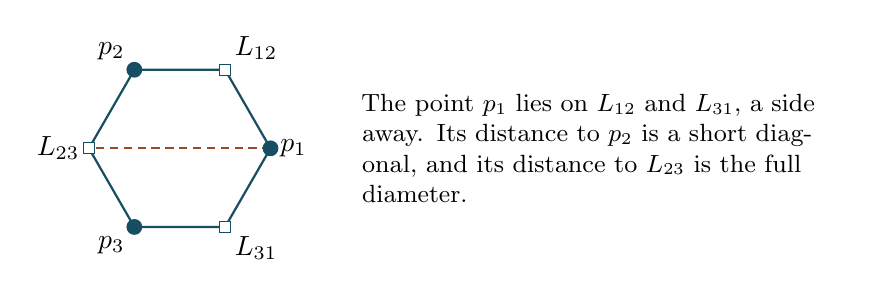
\begin{tikzpicture}[scale=1.02]
  \foreach \k in {0,...,5} \coordinate (h\k) at ({60*\k}:1.13);
  \draw[thick,inkblue] (h0)--(h1)--(h2)--(h3)--(h4)--(h5)--cycle;
  \draw[copper,thick,densely dashed] (h0)--(h3);
  \foreach \k in {0,2,4} \fill[inkblue] (h\k) circle (2.8pt);
  \foreach \k in {1,3,5} \node[draw=inkblue,fill=white,inner sep=2pt] at (h\k) {};
  \node[right] at (h0) {\(p_1\)};
  \node[above right] at (h1) {\(L_{12}\)};
  \node[above left] at (h2) {\(p_2\)};
  \node[left] at (h3) {\(L_{23}\)};
  \node[below left] at (h4) {\(p_3\)};
  \node[below right] at (h5) {\(L_{31}\)};
  \node[anchor=west,align=left,font=\small,text width=6.05cm] at (2.15,0)
    {The point \(p_1\) lies on \(L_{12}\) and \(L_{31}\), a side away.
     Its distance to \(p_2\) is a short diagonal, and its distance to
     \(L_{23}\) is the full diameter.};
\end{tikzpicture}
\end{center}

What needs proof is that the hexagons from \emph{different} bases agree
on their common terminals. There is no fixed basis containing all 21
points among its three coordinate axes. Appendix~\ref{app:plane} derives
the simultaneous placement from the Grassmannian argument of
\cite{euclid}. We can already use the table to design an experiment.

Put one binary wire on each incident point--line pair and call the
resulting tensor \(\src\). Put one wire on each nonincident point--line
pair and call this tensor \(\tgt\). There are \(21\cdot5=105\) wires in
the first tensor and \(21\cdot16=336\) in the second.

\begin{theorem}[A sufficient test for ports]\label{thm:six}
If there are local linear maps over \(F\) giving the restriction
\[
                            \src^{\otimes6}\res\tgt ,
\]
then \(F\) has ports.
\end{theorem}
\begin{proof}
Suppose \(F\) lacks ports and use the placement in
Proposition~\ref{prop:plane}. Each source wire has price one and each
target wire has price two. By \eqref{eq:graph-price} the proposed
restriction would turn a tensor of price \(6\cdot105=630\) into one of
price \(2\cdot336=672\). Monotonicity gives \(630\ge672\), a
contradiction.
\end{proof}

\paragraph{What would count as a solution?}
Each terminal receives six bits on each of five incident edges and must
produce one bit on each of sixteen nonincident pairs. Thus a solution is
42 matrices \(A_v:F^{2^{30}}\to F^{2^{16}}\). There is even an explicit
test for proposed matrices. For each terminal \(v\), choose a string \(y_v\)
of its sixteen output bits. Sum over assignments \(b\) of six bits to each
incidence edge. The required identity, for every choice of the \(y_v\), is
\begin{equation}
  \sum_b\ \prod_v A_v[y_v,b|_v]
  =\prod_{e=pL\ {\rm nonincident}}\one_{\{y_{p,e}=y_{L,e}\}} .
  \label{eq:witness}
\end{equation}
The tuple \(b|_v\) lists the thirty input bits seen at \(v\). On the right
each pair checks that its two output bits agree. This is a finite system
of polynomial equations with integer coefficients. An existence proof
could exploit the symmetries of the plane without printing the matrices.
As of \fieldstatus{}, the existence of these maps remains open. Failure
of this particular test leaves other ways for \(F\) to have ports.

\subsection{Two ways to test the proposed conversion}
\label{sec:cuts}

First try routing each target bit along a path of source edges. The
incidence graph is bipartite. A nonincident point and line are in opposite
parts, and any path joining them uses at least three edges. Even if we
split traffic fractionally, the 336 demands use at least \(3\cdot336=1008\)
edge units. Six copies of the source supply 630. Thus a construction at
the proposed rate has to use more of \eqref{eq:witness} than path routing.

Next try to disprove the conversion by flattening the tensor across a cut.
Equation~\eqref{eq:graph-price} reduces this test to counting edges. Here
the answer is quite different.

\begin{lemma}\label{lem:cuts}
For every cut of the 42 terminals, six times the number of crossing
incidences is at least the number of crossing nonincidences.
\end{lemma}
\begin{proof}
Write \(N\) for the real \(21\times21\) point--line incidence matrix.
Each point lies on five lines and each pair of distinct points shares one,
so \(NN^{\mathsf T}=4I+\one\one^{\mathsf T}\). On vectors orthogonal to
\(\one\), the singular values of \(N\) are all two.

Let \(u,v\) be the zero-or-one indicators of one side of the cut on
points and lines, respectively. Write \(u',v'\) for their mean-zero parts.
Set
\[
  T=\|u'\|^2+\|v'\|^2+21(\bar u-\bar v)^2,\qquad
  a=(u')^{\mathsf T}Nv'.
\]
The number of crossing incidences is \(\sum_{p,L}N_{pL}(u_p-v_L)^2\).
Expanding gives \(5T-2a\). For nonincidences the matrix is
\(\one\one^{\mathsf T}-N\), giving \(16T+2a\). Finally,
\(a\le2\|u'\|\|v'\|\le T\), whence
\[
                    6(5T-2a)-(16T+2a)=14(T-a)\ge0 .
\]
\end{proof}

The calculation is over the reals because it counts crossing edges.
Consequently the resulting flattening tests pass over every coefficient
field. The gap between the two computations leaves open whether local
linear combinations in \eqref{eq:witness} can use the available rank more
efficiently than routing the bits separately.

\paragraph{A ten-terminal variant.}
The same plane gives a different way to use the price table. Choose
distinct points \(P,Q\) and write \(PQ\) for their common line.
Form a list \(A\) from two copies of \(P\) and
the four lines through \(Q\) other than \(PQ\). Form \(B\) by exchanging
\(P\) and \(Q\). There are twelve list entries but only ten terminals.
Let \(S\) supply one wire between every entry of \(A\) and every entry of
\(B\), and let \(T\) demand one wire per unordered pair of entries within
each list. A wire from a terminal to itself can be discarded.

Within \(A\), eight point--line pairs are nonincident and six line pairs
have distance \(\sqrt3\). Between the lists, sixteen point--line pairs are
incident, and the four point pairs and sixteen line pairs have distance
\(\sqrt3\). Thus the forced placement gives
\[
            h(T)=32+12\sqrt3,\qquad h(S)=16+20\sqrt3
\]
in the common unit of Proposition~\ref{prop:plane}. The ratio exceeds
\(26/25\), so \(S^{\otimes26}\res T^{\otimes25}\) would also prove ports.
For a cut containing \(u\) entries of \(A\) and \(v\) of \(B\), the
number of crossing wires in \(S\) minus that in \(T\) is \((u-v)^2\).
Even a one-for-one conversion passes this cut test.

There is a geometric target here too. A distance table is of
\emph{negative type} if \(\sum_{i,j}c_i c_j d_{ij}\le0\) for every choice
of real \(c_i\) summing to zero. Give each terminal its multiplicity in
\(A\) minus its multiplicity in \(B\). The sum becomes
\(2(h(T)-h(S))=32-16\sqrt3>0\). Thus proving negative type
for all spectral wire distances in one characteristic would establish
ports there. This criterion concerns the unsquared wire distance.

\section{How to settle a characteristic}
\label{sec:decide}

The six-copy test is attractive because we can name the tensors. There
is also a search guaranteed to find \emph{some} finite certificate whenever
the answer is yes. The asymmetry between a yes and a no comes from the
order of the quantifiers in Definition~\ref{def:ports}.

\subsection{Amplifying one finite graph}

The following amplification theorem converts one finite success into a
family of successes. There is an absolute constant \(c>0\) such that if
\(F\) has no ports, then every connected \(d\)-regular graph on \(n\ge2\)
vertices satisfies
\begin{equation}
                 \Gamma_F(G)\ \ge\ c\,\frac{\log n}{\log(d+1)} .
                 \label{eq:log}
\end{equation}
This is the logarithmic Poincar\'e obstruction of \cite{circuits}. The
ratio of logarithms is independent of their base. The contrapositive says
that one graph beating this threshold \emph{uniformly over all placements}
proves ports. Roughly, the proof puts a copy of the good graph at each
vertex of a preceding graph. A short random walk among the old vertices
is used to join the copies. Under the threshold, the order grows at
each iteration while the comparison constant stays bounded. The related amplification in OpenAI~\cite[Section~11.1]{euclid} credits the balanced replacement product of Reingold, Vadhan and Wigderson~\cite[Definition~6.6]{rvw-zigzag} and the nonlinear product and walk estimates of Mendel and Naor~\cite[Theorem~1.13(V) and Section~8]{mn-nonlinear}\cite[Corollary~1.9]{mn-spectral}\cite[Theorem~3.4]{mendel}.

There is a useful purely algebraic consequence.
\begin{theorem}[One-sided search]\label{thm:search}
There is an effectively enumerable list of pairs of integer tensors,
independent of \(F\), with the following property. A characteristic has
ports if and only if at least one listed source restricts to its target
over the algebraic closure of its prime field.
\end{theorem}
The prime field is \(\mathbb Q\) in characteristic zero and \(\F_p\) in
characteristic \(p\). Its algebraic closure is the field obtained by
adjoining all algebraic roots. For each tensor pair, the entries of the
local maps are unknowns in polynomial equations, as in
\eqref{eq:witness}. Over an algebraic closure, Hilbert's Nullstellensatz
says the system is inconsistent exactly when a polynomial combination
of its equations gives \(1\). A Gr\"obner basis algorithm decides this
ideal-membership test. The enumeration therefore halts with a certificate
in every positive instance and may run forever in a negative one.
Appendix~\ref{app:search} constructs the list.

\paragraph{What a characteristic-zero witness would buy.}
A characteristic-zero certificate in Theorem~\ref{thm:search} has maps
over \(\overline{\mathbb Q}\). Their finitely many entries lie in a single
number field.
After clearing finitely many denominators, reduce the entries at a prime
ideal above \(p\). For all sufficiently large rational primes \(p\) this
gives local maps over \(\overline{\F}_p\). In the construction of
Appendix~\ref{app:search}, a successful test supplies a particular graph
and a uniform bound. The same graph and bound therefore work in all these
characteristics, and amplification gives a \emph{common port family}.
In particular, infinitely many prime characteristics without ports would
force characteristic zero to lack ports as well.

\subsection{Ruling out every bounded-degree family}

Fix a degree bound \(D\). To establish absence of ports one must show that,
as the order tends to infinity, even the \emph{best} allowed graph has an
unbounded worst-case ratio. Precisely, for every \(D\ge2\),
\[
 \lim_{N\to\infty}\
 \inf_{\substack{G\ {\rm connected,\ regular}\\ |V(G)|\ge N,\ \deg G\le D}}
             \Gamma_F(G)=\infty .
\]
Indeed, bounded ratios on graphs of arbitrarily large order give a port
family by selecting a subsequence. A bad placement may depend on \(G\).
The cycle cut disposes of every long cycle in one stroke. An expander has
many edges across every balanced cut and needs a different placement.

For a concrete target, give a connected graph \(G\) its shortest-path
distance \(\rho\), and try to realize \(d(u,v)=\sqrt{\rho(u,v)}\) as a wire
distance over \(F\). Edges then have squared length at most one. A ball of
integer radius \(r\) has at most \((D+1)^r\) vertices, by counting walks
and allowing holding steps. If this number is at most \(n/2\), at least
half the vertices have squared distance greater than \(r\) from any
fixed vertex. Thus \(\Var\ge r/2\). Realizing these distances, even up to
uniformly bounded multiplicative distortion and a common rescaling, on
all candidate graphs would prove a no. The open part of this proposal
is to produce the spectral prices witnessing those distances.

There is a geometric reason a no would be consequential. Spectral
distances extend to \emph{Hadamard spaces} \cite{euclid}. These are
complete metric spaces with shortest segments in which every midpoint
\(m\) of \(a,b\) satisfies the Euclidean midpoint inequality
\begin{equation}
 d(z,m)^2\le\tfrac12d(z,a)^2+\tfrac12d(z,b)^2-\tfrac14d(a,b)^2.
 \label{eq:midpoint}
\end{equation}
Euclidean space has equality. The inequality implies that segments are
unique. If a characteristic lacks ports, choose one witnessing placement
from \eqref{eq:log} for each finite connected regular graph, reducing
\(c\) by a factor of two if a supremum is only approached. There are
countably many graphs. Place their witness spaces in different coordinates
of a single product, with squared distances added and with points at
finite squared distance from a fixed basepoint. This product is complete
and satisfies \eqref{eq:midpoint} coordinatewise. Inside it, each graph
still has its bad placement. Thus one no-ports field would produce a
single Hadamard space admitting no bounded-degree expander sequence
relative to its metric, a question also studied independently of tensors
\cite{mendel,ann}.

\section{What changes over the complex numbers?}
\label{sec:flags}

The entries of the two graph tensors in Section~\ref{sec:experiment} are
zeros and ones. Characteristic enters through the local maps they admit.
A second approach exposes the coefficient field through the subspaces
of a vector space. This time the smaller plane of order two already
detects a difference.

A \emph{weighted flag} is a nested chain of subspaces with a real weight
on each successive layer. Equivalently, its subspace at threshold \(s\)
is spanned by the layers of weight at least \(s\). Two flags in \(K^h\)
have a common adapted basis, obtained by extending bases of their
intersections starting with the deepest pieces. If their weight lists in that basis are
\((a_j)\) and \((b_j)\), define
\[
                 d_{\rm fl}^2=\frac1h\sum_{j=1}^h(a_j-b_j)^2 .
\]
For increasing weight levels \(a_k,b_l\), let \(r_{kl}\) be the normalized
dimension of the intersection of the two threshold spaces. The fraction
of basis vectors carrying exactly \((a_k,b_l)\) is
\(r_{kl}-r_{k+1,l}-r_{k,l+1}+r_{k+1,l+1}\), with out-of-range entries
zero. Thus the distance depends only on the threshold intersections.

Over \(K=\F_2\), take the actual points and lines \(U\) of the plane in
\(\F_2^3\). Give \(U\) weight \(1-r/3\) and its quotient weight \(-r/3\),
where \(r=\dim U\). In a basis adapted to two subspaces, the weight vector
for \(U\) is its coordinate indicator minus \(r\one/3\). The same hexagon
calculation as in Appendix~\ref{app:plane} gives the full fourteen-site
table of Proposition~\ref{prop:plane}, up to scale. This is the unit-radius configuration in the cone on the Fano incidence graph studied by Izeki and Nayatani~\cite[Example~5 and Section~6]{izeki}. This constructs an
ordinary flag model for one necessary table. Ruling out ports over
\(\F_2\) would still require spectral witnesses against every candidate
graph family.

\begin{proposition}\label{prop:flags}
The fourteen-site table has a positive gap from all ordinary complex flag
tables, even allowing unbounded dimension and rescaling. More precisely,
each embedding into such flags has distortion at least
\(\sqrt{2(1-\sqrt2/3)}>1.028\), where distortion is the ratio of greatest
to least multiplicative change in a nonzero distance.
\end{proposition}
\begin{proof}
Let \(G\) be the incidence graph of the seven points and seven lines. Each
vertex has degree three. The incidence matrix satisfies
\(NN^{\mathsf T}=2I+\one\one^{\mathsf T}\), so the second eigenvalue of
the normalized adjacency of \(G\) is \(\lambda=\sqrt2/3\). The bipartite
graph of nonincidences is four-regular. Counting edges from any set of
points gives at least as many neighbors as points, so Hall's marriage
theorem gives a perfect matching \(M\). In the proposed table
each edge of \(G\) has length one and every pair in \(M\) has length two.

In a smooth Hadamard space the mean of squared
distances from finitely many sites has a minimizer \(b\), the
\emph{barycenter}. The tangent vectors \(v_i=\log_b x_i\), pointing from
\(b\) to the sites, have lengths \(d(b,x_i)\), have sum zero by first
variation, and satisfy \(\|v_i-v_j\|\le d(x_i,x_j)\) \cite{izeki}.
The Euclidean calculation in Section~\ref{sec:definition} and the triangle
inequality on matched pairs give
\[
 \E_{G}d^2\ \ge\ 2(1-\lambda)\E_i d(b,x_i)^2
       \ \ge\ \frac{1-\lambda}{2}\,\E_M d^2 .
\]
Here the subscripts denote a uniform directed edge, vertex, or matched
pair. Appendix~\ref{app:hermitian} explains why every finite table of
complex flag distances is a limit of rescaled distances in smooth
Hadamard spaces. The inequality therefore holds for these flags. Rescale
an embedding of distortion \(D\) to make its least expansion one. Its
edge average is at most \(D^2\) and its matched-pair average is at least
four. This gives \(D^2\ge2(1-\lambda)>1\).
\end{proof}

Why does this leave \(\mathbb C\) open? The exterior construction of
\cite{circuits} associates \emph{abstract} flags to a spectral cone, a
spectral space equipped with dilations from a distinguished origin.
Its thresholds come with a normalized dimension and operations of sum
and intersection satisfying rank--nullity. Pairwise threshold dimensions
define the flag distances, and the construction multiplies every original
distance by the same constant. In the forced plane all pairs of rays from
the center lie in a Euclidean piece. Magnifying about the center and
taking the limit therefore preserves the fourteen distances in a spectral
cone. A characteristic-zero field without ports would give fourteen
abstract exterior flags with exactly the forbidden table.

This leaves a specific algebraic question. Can the dimensions of the
thresholds and their pairwise intersections in such a witness be
approximated jointly by the thresholds of ordinary complex flags? It suffices to do
this at finitely many thresholds of each flag, since truncation and finer
discretization converge in the flag metric, whereas
Proposition~\ref{prop:flags} has a strict gap. A proof of this approximation
for every proposed witness, or a direct proof of the displayed
edge--matching inequality for the abstract flags, would establish ports
in characteristic zero. Joint approximation for these witnesses remains
open. The construction sought in \eqref{eq:witness} would settle a
characteristic directly from its allowed local linear maps.

\section{What ports would tell us about counting expanders}
\label{sec:patterns}

In Section~\ref{sec:definition} we chose a graph on attachment sites
to test all wire prices. Here we choose a graph \(H\) to count. Its
\(k=|V(H)|\) vertices include every vertex introduced by a construction.
The host has \(n\) vertices and one indeterminate \(X_{ij}\) per unordered
pair. The \emph{ordinary non-induced} polynomial sums over copies of
\(H\) in the complete host, counting each unlabelled copy once. Its term
is the product of the weights on the edges of the copy. For an
\emph{induced} count we also multiply by \(1-X_{ij}\) for every missing
edge on its vertices. For example, a path with edges \(ij,j\ell\)
contributes \(X_{ij}X_{j\ell}\) in the first count and
\(X_{ij}X_{j\ell}(1-X_{i\ell})\) in the second.

For either polynomial \(P_{H,n}\), let \(C_F(P_{H,n})\) be the fewest
binary addition, subtraction and multiplication gates computing it as a
formal polynomial over \(F\). Constants from \(F\) and reuse of gates are
allowed. Write its \emph{host exponent} as
\[
       a_F(P_H)=\liminf_{n\to\infty}
                      \frac{\log(1+C_F(P_{H,n}))}{\log n}.
\]
We first hold \(H\) fixed and let the host grow, then compare exponents
along families with \(k\to\infty\). Thus even \(2^k\) calls to a circuit
cost only a constant factor in the first limit.

\paragraph{If the characteristic has no ports.}
The following are lower bounds on \(a_F(P_H)\). Each row describes a
family of expanders. A proof of absence in characteristic two, for
example, would give all three bounds over \(\F_2\) and every extension.
The classification is open even for \(\F_2\) and \(\mathbb C\).
\begin{center}
\begin{tabular}{@{}lll@{}}
\toprule
Pattern family & Copies counted & Lower bound if \(F\) has no ports\\
\midrule
Maximum degree six & Induced & \(\Omega(k/\sqrt{\log k})\)\\
Edge density tending to \(1/4\) & Non-induced & \(\Omega(k/\sqrt{\log k})\)\\
Bounded degree & Non-induced & \(\Omega(k/(\log k)^{17/2})\)\\
\bottomrule
\end{tabular}
\end{center}

To see where the first row comes from, start with the exterior tensor
in the no-ports proof of \cite{circuits}. Its \(d\) rows make \(d\)
choices. A nonzero coefficient is a signed product of Vandermonde
differences \(\xi_j-\xi_i\). Each factor sees at most two row choices.
The signs also factor over pairs. Recording a running count of occupied
slots in each row lets consecutive rows check the required totals.
Thus one vertex from each of \(d\) classes can record all the choices.
The product of the clique edge weights gives their coefficient. Putting
each row variable on the edge to the next class in cyclic order also
supplies the monomial for that tuple. The
quantitative point is the cost of recording a choice. For \(h\) tensor
copies, a class needs at most \(\exp(O(hw))\) vertices, where \(w\)
is the row-width parameter. The tensor polynomial requires
\(\exp(\Omega(hwd/\sqrt{\log d}))\) gates. Taking logarithms and
letting \(h\) grow gives a host exponent \(\Omega(d/\sqrt{\log d})\)
for colorful \(d\)-clique, which selects one vertex from each class.
Unused host vertices can be padded by isolates between successive
powers. The pair weights may be chosen in an extension of \(F\), since
any circuit over \(F\) also works there. See the detailed reduction
in \cite{pairtables}.

Now take a cubic expander on \(r\) vertices. Keep its edges and add
one new vertex adjacent to both ends of each edge. The enlarged graph
is an expander of maximum degree six. The \(d=3r/2\) new vertices
are independent, and \(k=r+d\), so \(d=3k/5\). In the host, give
each old vertex a singleton class and each new vertex a class of
choices. Inclusion--exclusion forces the \(r\) singletons into the
copy. Make each class of choices a clique and give pairs in distinct
choice classes weight \(1-Y_{ij}\). Fix adjacencies to the singletons
as prescribed by the pattern. If the \(d\) independent positions used
\(a>0\) singletons, the incident base edges would exclude at least
\(3a/2\) choice classes. Each remaining class supplies at most one
independent vertex, giving fewer than \(d\) in all. Hence those
positions take exactly one choice from each class. Their
missing edges then contribute \(1-(1-Y_{ij})=Y_{ij}\), exactly the
colorful clique factors. This uses at most \(2^r\) evaluations on a
host growing linearly with the clique host. Substituting \(d=3k/5\)
therefore preserves the order of the clique exponent \cite{sparse-patterns}.

For the dense non-induced family a different reduction retains a clique
on \((k-O(\log k))/2\) positions \cite{pairtables}. For the bounded-degree
non-induced family, the construction evaluates the same exterior minors
by local operations and routes their inputs through a bounded-degree
graph. It uses \(k=O(d(\log d)^8)\) vertices. Charging those vertices
explains the exponent \(8+1/2=17/2\) in the third row \cite{sparserouting}.

\paragraph{If the characteristic has ports.}
The network compression from Section~\ref{sec:cycle} enters a different
lower-bound proof. It gives \(2^{t^{\varepsilon}}\) as a lower bound
for directed Hamiltonian cycle on \(t\) vertices, with some
\(\varepsilon>0\) depending on the characteristic, and the same bound
for the \(t\times t\) permanent outside characteristic two \cite{circuits}.
This can also give expander bounds when the pattern grows with the
host. For example, a colorful clique can encode a tour by choosing
its successive, distinct vertex labels in \(t\) classes, with the first
label fixed. The arc weights go between successive classes. Putting
this clique into an expander count takes at least \(t\) pattern
positions. For example, on particular sparse induced expanders and
their dense non-induced complements with \(k=n^{1/2+o(1)}\), the two
branches together give \(n^{\Omega(\log n/(\log\log n)^2)}\) gates
over every field \cite{pairtables}. With \(k\) fixed the tour order
stays bounded as \(n\) grows, so the tour projection alone yields no
positive host exponent.

\paragraph{How far from \(\boldsymbol{n^{ck}}\)?}
Over \emph{every} field, for each \(\varepsilon>0\) there is an explicit
bounded-degree expander family whose ordinary non-induced exponent is
at least \((1/\sqrt{2}-\varepsilon)\sqrt{k}\). There is also an
all-fields upper bound \(O(k/\sqrt{\log k})\) on the upper limiting
exponent for every ordinary non-induced family with \(O(k)\) edges
\cite{sparse-patterns}. Dividing by \(k\) shows that these sparse counts
rule out \emph{every} fixed \(c>0\), whichever answer their field gives
to the ports question.

Dense non-induced counts and sparse induced counts still leave room
for a fixed \(c>0\). The first two rows of the table give only a
coefficient of order \(1/\sqrt{\log k}\) in front of \(k\). In
characteristic zero one can state the outstanding induced question
particularly sharply. The top homogeneous part of the induced
\(H\)-polynomial is the \(k\)-clique polynomial times
\((-1)^{\binom{k}{2}-|E(H)|}k!/|\operatorname{Aut}(H)|\):
on each \(k\)-set every copy gives the same top monomial. The scalar
is nonzero, and interpolation extracts this part at cost depending
only on \(k\) per gate. Conversely, a colorful \(k\)-clique sum
computes the induced count by using \(X_{ij}\) or \(1-X_{ij}\) on
each pair of positions, forbidding repeated labels and dividing by
the number of automorphisms. A colorful clique sum is itself an ordinary
clique sum on a multipartite host with independent classes, since every
contributing clique takes one vertex per class \cite{pairtables,sparse-patterns}.
Thus even for induced
cubic expanders in characteristic zero, proving an exponent \(ck\)
amounts to proving that rate for \(k\)-clique.

There is a numerical ceiling on this approach. Split the \(k\) clique
positions into three groups of at most \(\lceil k/3\rceil\). One label
per group records all its vertex choices. After absorbing within-group
weights into the three pair tables \(A,B,C\), the clique sum is
\(\operatorname{tr}(ABC)\). The tables have side at most
\(n^{\lceil k/3\rceil}\), so square matrix multiplication bounds the
asymptotic coefficient by \(\omega_F/3=3/4\) \cite{matrix-exponent}. Whether even
one positive constant is attainable remains open here. No step in the
no-ports transfer assumes that the permanent needs \(2^{(1-o(1))t}\)
gates. Curticapean's algorithm rules out that premise for the generic
\(t\times t\) permanent even in characteristic zero \cite{stars}.

\appendix
\section{Why absence of ports forces the plane}
\label{app:plane}

The main geometric input is an equality case. For \(m\ge4\) a power of two,
let \(\Gr(m,2m;2)\) be the finite set of \(m\)-dimensional subspaces of
\(\F_2^{2m}\). Assign its members to sites in a spectral space over the
coefficient field \(F\). Two members are \(r\) steps apart in the
Grassmann graph if their intersection has dimension \(m-r\). Let \(B_r\)
be the mean squared wire distance over ordered pairs at \(r\) steps.
In particular \(B_1\) measures the cost of changing one direction and
\(B_m\) measures the cost of changing all of them.

\paragraph{The Grassmannian input.}
The proof in \cite{euclid} gives \(B_{r+s}\le B_r+B_s\) for
\(r+s\le m\). A uniform strict improvement \(B_m\le(m-\eta)B_1\) for any
\(\eta>0\) and this fixed \(m\) implies ports. To see the role of strictness,
the Grassmannian construction in that proof uses the gain to produce
sparse symmetric transition matrices on \(D^{m^j}\) vertices, with row
support at most \(C_jD\) and comparison constant at most \(C'\alpha^j\),
where \(\alpha<m\). Here \(D\) can be any sufficiently large power of two.
The sparse-matrix version of \eqref{eq:log} in \cite{circuits} bounds this
constant below by \(c m^j\log D/\log(C_jD+1)\) in a class without ports.
First take \(j\) large and then \(D\) large relative to \(C_j\). The two
bounds are incompatible. This argument uses only the numerical gain.

Here is the geometry behind the factor \(m\). From
\eqref{eq:midpoint} one obtains the quadrilateral inequality
\[
 d(a,c)^2+d(b,d)^2\le
 d(a,b)^2+d(b,c)^2+d(c,d)^2+d(d,a)^2 .
\]
Take four subspaces \(K+R_i+S_j\), \(i,j\in\{0,1\}\), where
\(K,R_0,R_1,S_0,S_1\) are in direct sum and have dimensions
\(m-r-s,r,r,s,s\). In cyclic order their sides change \(r,s,r,s\)
directions, and both diagonals change \(r+s\). A uniform random invertible
linear change of coordinates makes each pair uniform among pairs of its
type. Averaging the quadrilateral inequality gives the claimed
subadditivity and hence \(B_r\le rB_1\).

If \(F\) lacks ports, there are placements with \(B_1=1\) and \(B_m\)
arbitrarily close to \(m\). All their entries are bounded since the set
of pairs is finite. The closure theorem for spectral distance tables
realizes a subsequential limit, up to a common change of scale
\cite{euclid}. At equality \(B_r=r\), because
\(B_m\le B_r+B_{m-r}\). We use the equality statement proved in the
Grassmannian argument, which gives squared distance \(r\) for every
\emph{individual} pair at \(r<m\) steps. Each quadrilateral deficit is
nonnegative while its average is zero. All quadrilaterals used in the
averaging thus have equal opposite sides. Changing one basis vector at
a time transports this equality between any two pairs at the same
proper distance \(r\). The restriction \(r<m\) leaves room for a spare
basis vector in this transport.

\paragraph{All ranks in one table.}
Let \(V=\F_{2^a}^{\,3}\) with \(a=1\) or \(2\). For a subspace \(U\le V\),
write \(U^\circ\le V^*\) for the linear functionals vanishing on \(U\).
Send \(U\) to \(U\oplus U^\circ\le V\oplus V^*\). Its dimension is
always three over \(\F_{2^a}\). The intersection codimension of the images
of \(U\) and \(W\) is
\[
          \dim U+\dim W-2\dim(U\cap W),
\]
since \(U^\circ\cap W^\circ=(U+W)^\circ\). Viewing all spaces as binary
vector spaces multiplies every dimension by \(a\). Choose \(m>3a\) a
power of two, embed \(V\oplus V^*\) into \(\F_2^{2m}\), and append the same
independent \((m-3a)\)-space to every image. The images now have rank
\(m\) and their pairwise intersection codimensions are at most \(3a<m\).
Apply the individual-pair equality and divide distances by \(\sqrt a\).
We obtain a single spectral placement of all subspaces with
\begin{equation}
                 d(U,W)^2=\dim U+\dim W-2\dim(U\cap W).
                 \label{eq:lattice}
\end{equation}

\paragraph{Centering the cubes.}
A basis of \(V\) picks out the eight subspaces spanned by subsets of that
basis. In \eqref{eq:lattice} their squared distances count differing
coordinates, exactly as on the corners of a Euclidean unit cube. The
cube-filling theorem of \cite{euclid} identifies their convex hull in
the spectral space with that cube. All cubes have the same corners \(0,V\)
at the ends of their long diagonal. Write \(o=\one/2\) for its midpoint
in cube coordinates.

For a point or line \(U\) of dimension \(r\), choose a basis containing a
basis of \(U\) and put
\[
         x_U=o+\tfrac12 w_U,\qquad w_U=\one_U-\tfrac r3\one ,
\]
where \(\one_U\) indicates the coordinate axes spanning \(U\). This site
has barycentric coefficients \(r/6,\ 1/2-r/6,\ 1/2\) on the three
corners \(0,V,U\). We can therefore construct it by first interpolating
on the common segment \(0V\) and then taking a midpoint with \(U\).
Uniqueness of segments makes it independent of the chosen cube.

To obtain a common adapted basis for two subspaces, extend a basis of
their intersection in each and complete to \(V\). In the corresponding cube,
\[
       \|w_U\|^2=2/3,\qquad
       \langle w_U,w_W\rangle=\dim(U\cap W)-\dim U\,\dim W/3 .
\]
In units for which \(d(o,x_U)=1\), distances are multiplied by
\(\sqrt6\). For distinct objects of the same type the unit vectors have
inner product \(-1/2\). For a point and a line it is \(1/2\) when incident
and \(-1\) otherwise. Their squared distances are \(3,1,4\), respectively.
This proves Proposition~\ref{prop:plane}.

\section{Why a positive answer has a finite certificate}
\label{app:search}

We prove Theorem~\ref{thm:search}. There are two finiteness issues.
Amplification deals with the infinitely many graph orders. Strict
spectral comparison deals with the infinitely many spectral points even
on one fixed graph.

\paragraph{The graph parameters.}
Enumerate connected regular multigraphs \(G\), rational \(\beta\ge1\),
and even \(t\) with
\[
                (2d+1)^t\le n/2,\qquad t\ge16384\beta .
\]
The proof of the logarithmic obstruction in \cite{circuits} shows that
\(\Gamma_F(G)\le\beta\) for one such choice gives a port family. For
clarity, its walk-smoothing estimate gives a bound
\(96(1+\gamma/t)\) from a previous graph of bound \(\gamma\). Rounding
the transition matrix doubles this to \(\rho=192(1+\gamma/t)\).
The replacement graph has mean edge energy
\((E_{\rm in}+E_{\rm match})/2\), half from the copies of \(G\) and half
from a matching between copies. The variance estimate in that proof is
at most \((6+18\rho)\beta E_{\rm in}+9\rho E_{\rm match}\).
Hence its bound is at most \(8192\beta(1+\gamma/t)\). Starting with one
vertex, iteration keeps the bound at most \(16384\beta\) on graphs of
orders \(n^j\) and degree \(2d\). Conversely, a port family contains
such a graph with \(\Gamma_F(G)<\beta\) once \(\beta\) is chosen strictly
above the uniform bound and \(n\) is sufficiently large.

\paragraph{A strict inequality on a compact set.}
Put \(z_{ij}=\phi(W_{ij})\in[1,2]\), since \(1\oplus1\res W_{ij}\res1\).
The possible \(z\)-tables form a compact set \cite{euclid}. Indeed the
prime field's algebraic closure is countable, so its finite tensors can
be enumerated. Each \(\phi(T)\) is bounded by the number of nonzero
entries of \(T\), since that many units in direct sum supply \(T\).
A diagonal subsequence of any sequence of spectral points converges on
all tensors. The limits satisfy the spectral axioms, giving the desired
compactness on the finitely many wire coordinates.

On the full cube of \(z\)-tables set
\[
          f(z)=\Var(\log_2 z)-\beta\En_G(\log_2 z),
\]
setting diagonal distances to zero. On the normalized spectral tables
\(\En_G>0\). In fact the wires of a spanning tree of \(G\) supply one
binary label shared by all sites. At every vertex keep equal incident
bits and discard inconsistent labels. The resulting tensor is \(1\oplus1\)
and has price one. Thus the tree edges cannot all have price zero.
For a graph with \(\Gamma_F(G)<\beta\), compactness now gives
\(\max_\phi f(z(\phi))<0\).

\paragraph{Turning the inequality into tensors.}
Choose a positive dyadic rational \(\epsilon\) and compute a rational
polynomial \(h\) approximating \(f\) with error at most \(\epsilon\) on the
whole cube. For instance expand \(\log z\) around \(3/2\), where
\(|(z-3/2)/(3/2)|\le1/3\), and bound the tail geometrically.
Clear positive denominators in \(h+2\epsilon\) and write the result as
\(P_+-P_-\) with nonnegative integer coefficients. Replace each variable
by its binary wire, multiplication by tensor product, and addition by
direct sum. This builds two tensors
\[
                       X=1\oplus P_+(W),\qquad Y=1\oplus P_-(W).
\]
They have integer entries and are nonzero. The inequality
\(\phi(X)\le\phi(Y)\) implies \(h(z)+2\epsilon\le0\), hence
\(f(z)\le-\epsilon\). Conversely, if \(\max_\phi f<0\), sufficiently small
\(\epsilon\) gives \(\phi(X)<\phi(Y)\) for every spectral point.

The last step uses strict spectral comparison \cite{strassen-spectrum,euclid}.
If \(A,B\ne0\) and \(\phi(A)<\phi(B)\) everywhere, there is an integer
\(K\) such that \(K B^{\otimes m}\res A^{\otimes m}\) for every \(m\).
Here \(K B\) denotes \(K\) copies in direct sum. In our strictly separated
case compactness gives \(\ell\) with \(2\phi(X)^\ell<\phi(Y)^\ell\)
everywhere. Apply comparison with \(A=2X^{\otimes\ell}\) and
\(B=Y^{\otimes\ell}\), then take \(m\) large enough that \(2^m>K\).
This produces a single ordinary restriction of the form
\[
                  K Y^{\otimes M}\res L X^{\otimes M},
                  \qquad 1\le K<L .
\]
Conversely, any such restriction forces \(\phi(X)<\phi(Y)\) throughout
the spectrum. Enumerate the graph parameters, the precisions and all
positive integers \(K,L,M\) with \(K<L\), by increasing total encoding
length. A success gives the required energy bound. The strict separation
argument guarantees a success somewhere on the list if the field has
ports. Scalar extension preserves the port property, so the search may
use the algebraic closure. This proves the theorem.

\section{Approximating complex flags by Hermitian forms}
\label{app:hermitian}

For the geometric input in Proposition~\ref{prop:flags}, use the space of
positive definite Hermitian forms on \(\mathbb C^h\). With its usual
invariant metric, normalized here by
\[
  d(H,K)^2=\frac{1}{4h}\sum_{j=1}^h
                 \bigl(\log\lambda_j(H^{-1}K)\bigr)^2 ,
\]
it is a smooth Hadamard space. All the eigenvalues in this expression are
positive. The realization of weighted flags at infinity in this space
is classical \cite{cornut}. The finite-table limit follows by choosing
adapted bases.

For each flag choose an adapted basis. At time \(t\) make its basis
vectors orthogonal and give a vector of weight \(a\) length \(e^{-ta}\).
Changing to another adapted basis for the same flag moves the resulting
form by \(O(1)\) distance, uniformly as \(t\to\infty\). Indeed a vector
of weight \(a\) is replaced by a linear combination of vectors of weights
\(b\ge a\). In rescaled coordinates the change-of-basis entries acquire
factors \(e^{-t(b-a)}\). The change of basis and its inverse are both
bounded, which bounds the log eigenvalues in the distance formula.
For a pair of flags use a common adapted basis. Their two forms are then
diagonal, and their distance divided by \(t\) is exactly
\(\big(h^{-1}\sum_j(a_j-b_j)^2\big)^{1/2}\). Returning to the original
bases changes the divided distance by \(O(1/t)\). With finitely many
pairs the errors tend to zero simultaneously, as required.

\begingroup\small
\bibliographystyle{../linkedtitles}
\bibliography{../references}
\endgroup
\end{document}
